  %-------------------------------------------------------------------------------
  %	SECTION TITLE
  %-------------------------------------------------------------------------------
  \cvsection{Projects}


  %-------------------------------------------------------------------------------
  %	CONTENT
  %-------------------------------------------------------------------------------
   \cvsubsection{Project\#1}

   %---------------------------------------------------------
    \cvparagraph
    {
      \begin{wrapfigure}{r}{0.5\textwidth}
        \centering
        \vspace{-10pt}
        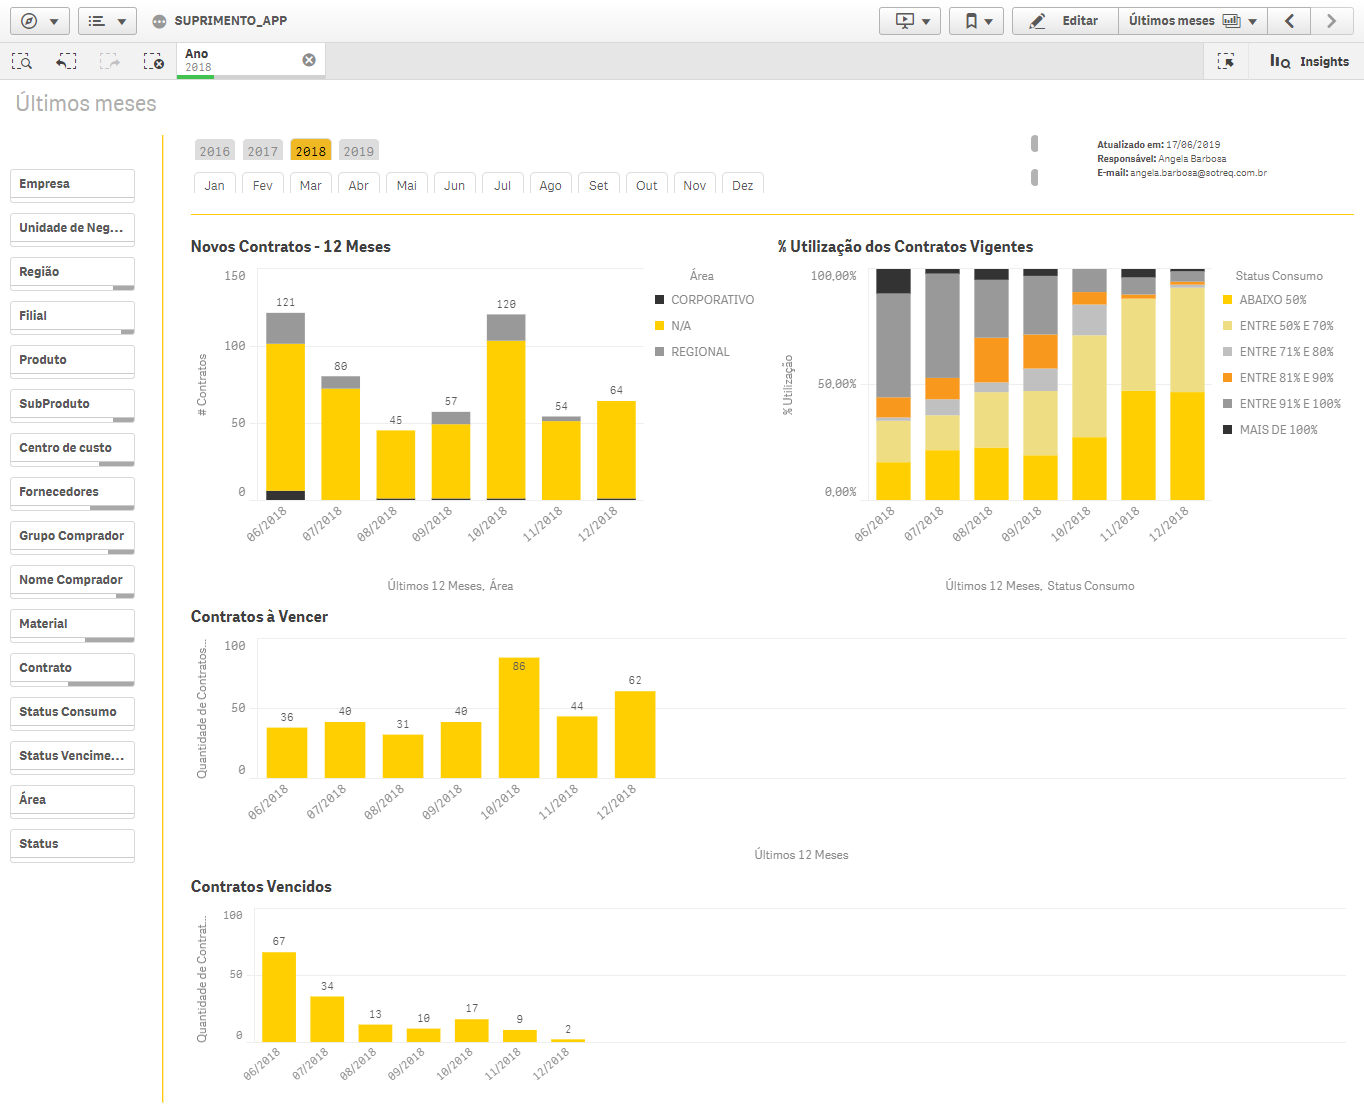
\includegraphics[width=0.5\textwidth]{img/project2}
      \end{wrapfigure}
      An engineering machinery company kept all of its supplier's contract data in the SAP system, it must somehow audit these contracts.

      Data was extracted from SAP using Qlik View's own language and a special connector provided by the software. These data were modeled and presented in the Qlik Sense tool.

      \textsc{Techonologies used}: Qlik View, Qlik Sense.
      \vfill
    }

  %---------------------------------------------------------

  \cvsubsection{Project\#2}

  %---------------------------------------------------------
    \cvparagraph
    {
      \begin{wrapfigure}{r}{0.5\textwidth}
        \centering
        \vspace{-10pt}
        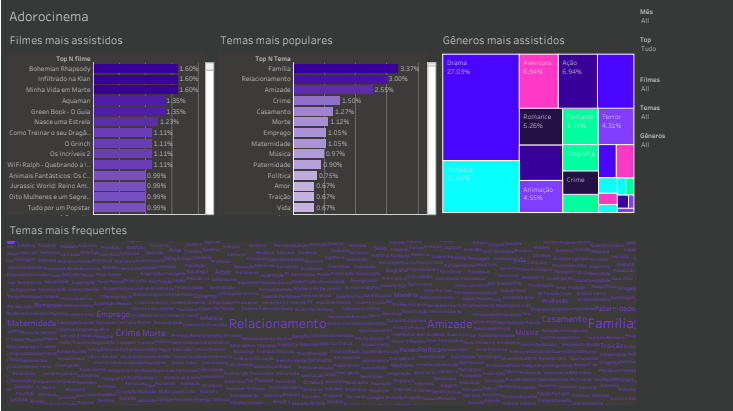
\includegraphics[width=0.5\textwidth]{img/project1}
      \end{wrapfigure}
      A marketing and advertising company needed dashboards to track social networking data, which was enriched by its employees by adding keywords using Google sheets.

      When I started the project, my role was to create database model and dashboards but there was legacy python code from which I made improvements by adding a database management framework (ORM). Later, there was a need of database migration, confirming the right decision to add an ORM.

      \textsc{Techonologies used}: Python, SQL Alchemy, SQL Server, Postgres, Api Google Docs, Tableau.
      \vfill
    }

  %---------------------------------------------------------

    \cvsubsection{Project\#3}

    %---------------------------------------------------------
     \cvparagraph
     {
      \begin{wrapfigure}{r}{0.5\textwidth}
        \centering
        \vspace{-10pt}
        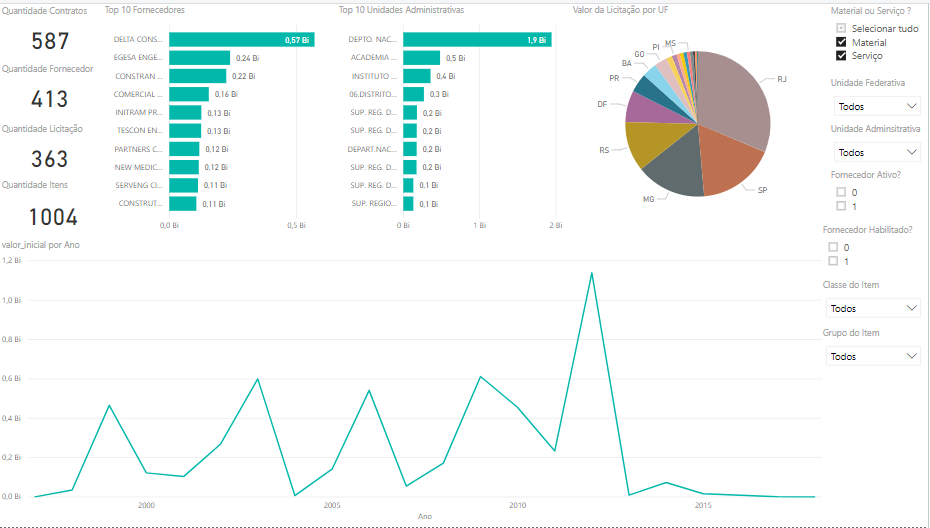
\includegraphics[width=0.5\textwidth]{img/project3}
      \end{wrapfigure}
      This was one of my projects for the MBA in Business Intelligence, where I compiled public procurement data from Brazilian government.

      The data was consumed through a web API, generating flat files. These files were inserted into database and made available by a visualization tool.

      Over time I have intention to make this vision available to the Brazilian population.

      \textsc{Techonologies used}: Pentaho, Postgres, Power BI
      \vfill
    }
   %---------------------------------------------------------
